\documentclass[12pt, a4paper, onecolumn]{article}
\usepackage{fontspec}
\usepackage{titlesec}
\usepackage{tocloft}
\usepackage[english]{babel}
\usepackage{blindtext}
\usepackage{subfig}
\usepackage{pgf}
\setmainfont{Georgia}

\newcommand\sectionfont{\normalfont\fontspec{Arial}\fontsize{14pt}{0}\bfseries}
\newcommand\subsectionfont{\normalfont\fontspec{Arial}\fontsize{13pt}{0}\bfseries}
\newcommand\subsubsectionfont{\normalfont\fontspec{Arial}\fontsize{12pt}{0}\bfseries}
\newcommand\tocsectionfont{\normalfont\fontspec{Arial}\fontsize{12pt}{0}\bfseries}
\newcommand\tocsubsectionfont{\normalfont\fontspec{Arial}\fontsize{11pt}{0}\bfseries}
\newcommand\tocsubsubsectionfont{\normalfont\fontspec{Arial}\fontsize{11pt}{0}}
\newcommand\toctitlefont{\normalfont\fontspec{Arial}\fontsize{16pt}{0}\bfseries}

\titleformat{\section}{\sectionfont}{\thesection}{20pt}{}
\titleformat{\subsection}{\subsectionfont}{\thesubsection}{20pt}{}
\titleformat{\subsubsection}{\subsubsectionfont}{\thesubsubsection}{20pt}{}

\renewcommand{\cftsecfont}{\tocsectionfont}
\renewcommand{\cftsubsecfont}{\tocsubsectionfont}
\renewcommand{\cftsubsubsecfont}{\tocsubsubsectionfont}
\renewcommand{\cftsecpagefont}{\tocsectionfont}
\renewcommand{\cftsubsecpagefont}{\tocsubsectionfont}
\renewcommand{\cftsubsubsecpagefont}{\tocsubsubsectionfont}
\renewcommand{\cfttoctitlefont}{\toctitlefont}

\addto\captionsenglish{
	\renewcommand{\contentsname}{Table of Contents}
}

\begin{document}
	
	\title{An accurate smart phone based fall detection system}
	\maketitle

	\tableofcontents
	\newpage
	
	\section{Introduction}
	
		\subsection{Background}
		
		\paragraph{Accidents related to falling} is a major issue in our society. In fact, according to the World Health Organization, "Falls are the second leading cause of accidental or unintentional injury deaths worldwide" \cite{who}. Globally, an average of 37.3 million people (Jan 2018) suffer from injuries related to a fall each year, which are severe enough to seek medical attention. Out of these, no less than an estimated 640 000 individuals die as a direct consequence of the fall \cite{who}. Fall  related accidents are therefore to be considered as a significant world wide health problem. 
		
		\paragraph{Although Age} is identified as a key driving factor behind fall related injuries, it is not by far the only reason that people hurt them selves this way every year.  Other risk factors include 
		\begin{itemize}
			\item Occupations which require you to work at an elevated height.
			\item Alcohol and substance abuse.
			\item Medical conditions contributing to a reduced sense of balance or vision.
			\item Sporting.	
		\end{itemize}
		
		\paragraph{In Sweden} alone, statistics shows even darker figures. Here, falling is the single one reason responsible for the greatest number of accident related fatalities, hospitalizations, and visits to emergency clinics, outnumbering traffic accidents, who come in second \cite[p~3,5]{msb_report}. On top of that, in Sweden, falling is together with poisoning, the type of accident who poses the biggest annual growth, having duplicated the amount of yearly incidents since 2000 \cite{soc_olyckor} Studies have also showed that peoples perception target traffic accidents as the the most common cause of the above \cite[p~5]{msb_report}. That is however not true, but a reasonable explanation for this is according to MSB (Swedish Civil Contingencies Agency) that most fall related accidents happen in a domestic area and are thus not as dramatic as a car accident or a fire for example. This tend to give this type of accident less space in the common media. 
		
		
		\paragraph{}The work force is by no means an exception to the statistics presented above in Sweden. The swedish work environment authority (Arbetsmiljöverket) published a study in 2016, claiming that fall accidents are the most versus second most common reason for absence in work due to accident, for women and men respectively \cite[p~1]{av}. This does not only have an impact on the lives of the individual and his or her family, it also poses serious economical damage to the society in general, and the affected organizations in particular. The diagram below illustrated the amount of fall related accidents in the most affected occupations. 
		
		
		\begin{figure}[h]
			\centering
			\subfloat[label 1]{{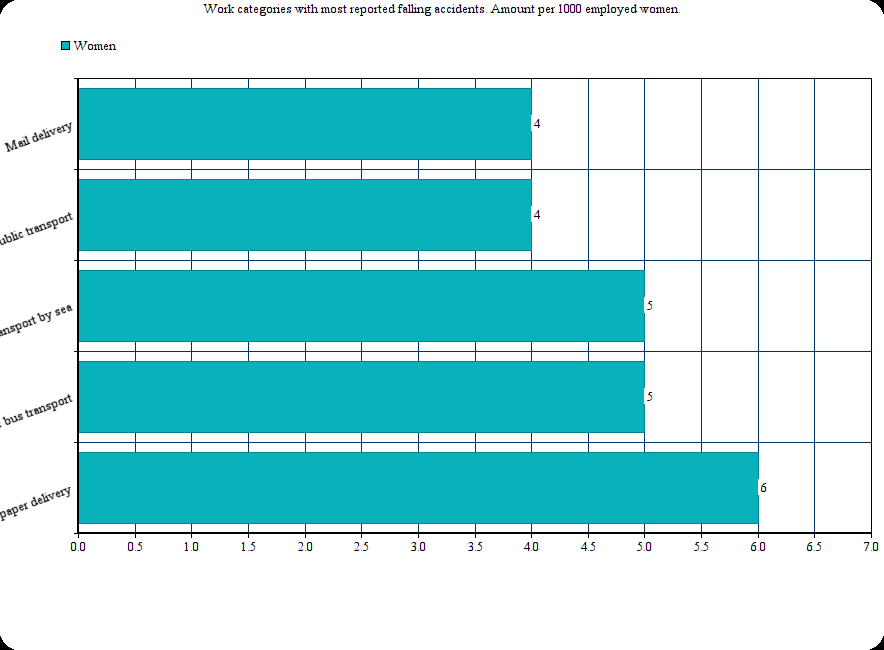
\includegraphics[width=6cm]{../img/Fall_from_ground_women.png} }}%
			\qquad
			\subfloat[label 2]{{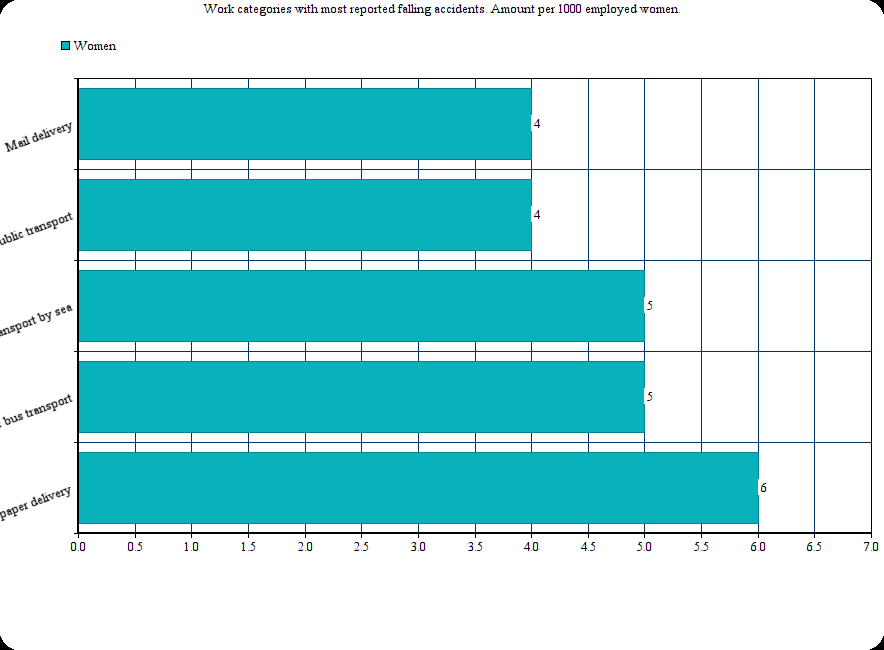
\includegraphics[width=6cm]{../img/Fall_from_ground_women.png} }}%
			\caption{Män och kvinnor som faller från stående höjd}%
			\label{fig:example}%
		\end{figure}
		
		\begin{figure}[h]
			\centering
			\subfloat[label 1]{{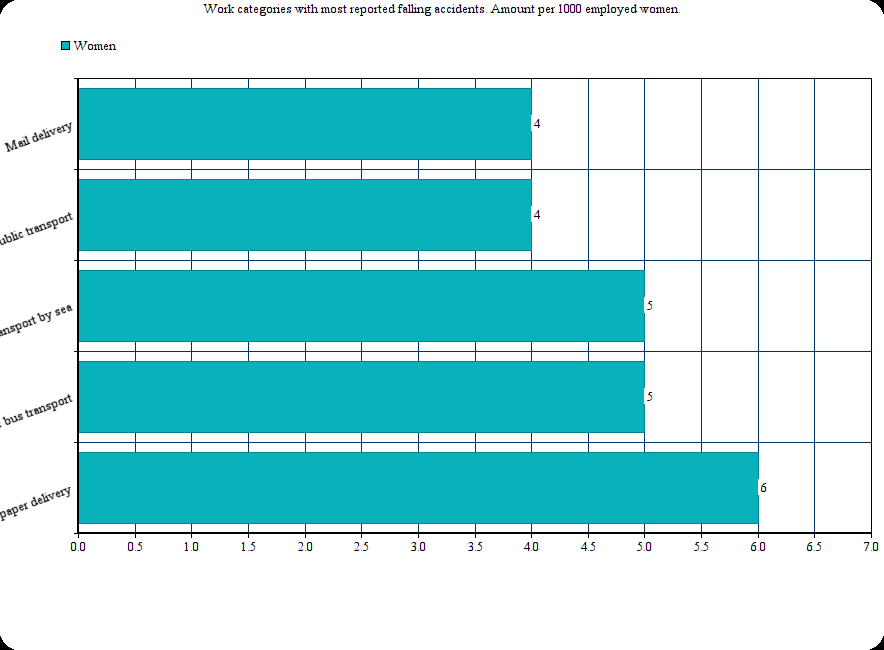
\includegraphics[width=6cm]{../img/Fall_from_ground_women.png} }}%
			\qquad
			\subfloat[label 2]{{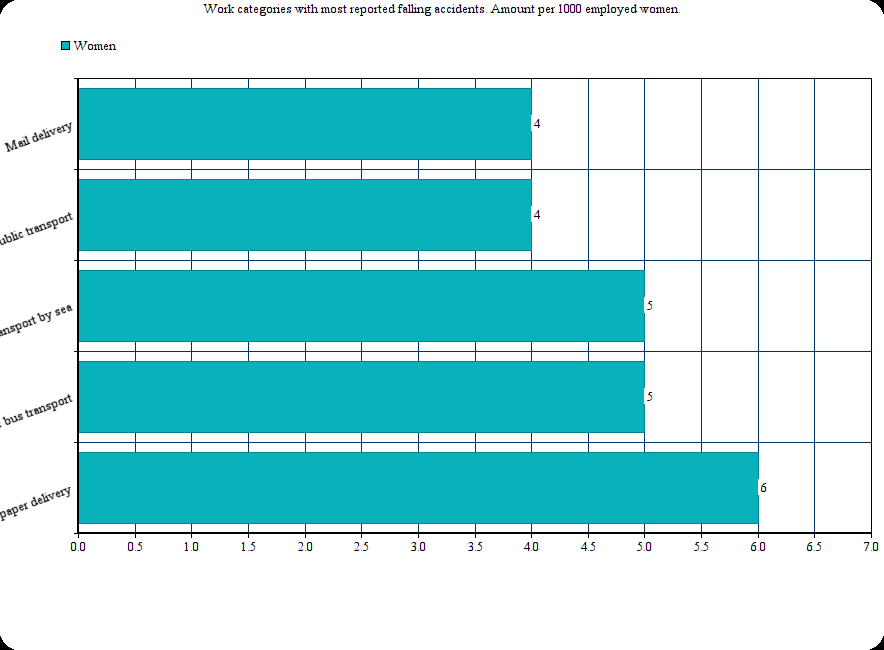
\includegraphics[width=6cm]{../img/Fall_from_ground_women.png} }}%
			\caption{Män och kvinnor som faller från eleverad höjd}%
			\label{fig:example}%
		\end{figure}
		
		\subsection{Problem}
		
		Since falling accidents are common, as described in the background, we want to examine the possibility of creating a mobile application that can detect falling accidents and inform registered contacts. This kind of application could help the person that suffer a falling accident by automatically contacting people that can come to aid the affected person. In case the person who have been involved in the fall is injured or unconscious and unable to call for help, the application will assist the person by automatically sending an alarm.
		
		\subsubsection{Q1}
		What algorithm should be used to accurately detect a fall?
		
		\subsubsection{Q2}
		How can technology available in smart phones be used to implement this algorithm?
		
		\subsubsection{Q3}
		How can performance issues be minimized when using the above technologies?
		
		\subsection{Purpose}
		
		The purpose of the thesis is to present the work conducted in the project, and give an answer to the questions formulated.
		
		The purpose of the project is to examine the possibility of using a mobile phone's embedded accelerometer to detect falling accidents.
		
		\subsection{Goal}
		
		The goal of the project is to create an application that, in an effective way, can detect falling accidents and inform concerned contacts. This application should target employees in fields such as operations, construction, etc., and should run in the users cell phone. The user of the application should be able to register contact information to relatives, colleagues, etc. After that the user can activate the protection in the application by selecting the appropriate option, for example by pressing a button in the application. The user is supposed to do this before starting a critical operation such as performing work on an elevated height or similar. When the protection in the application is activated the application makes use of the device's embedded accelerometer to register changes in velocity. If the user would carry the device running the application with the protection actived, while the user would suffer a falling accident, the application would detect this and enter a warning state. In the warning state the application will notify the user that a fall has been detected and that the application soon will send an alarm to registered contacts. If the time limit for the warning state exceeds without any action from the user, an alarm will be sent to the registered contacts using for example SMS.
		
		According to the company that we will work together with, the most important feature is fall detection. It is important that we develop both an Android implementation and an iOS implementation. If we suffer from a lack of time we will not prioritize user interfaces and integration with other functionality, but focus on fall detection. The project will be reported to the company by handing over a GitHub repository.  
		
		\subsubsection{Sustainability \& Community benefits}
		
		Since the application will not replace any existing technology it is difficult to discuss in which way the application will affect the environment. Our project will be focusing on software alone and will only use hardware that already exists, and thus it will not affect the environment in greater extent. You could however argue that since the application will run on a cell phone, that will draw more current if it runs an additional application in the background, our project will affect the environment but it is hard to say how great such an effect will be.
		
		From a social perspective we hope that the application will contribute to the society in a positive way, since the intention is that the application will help to minimize the negative consequences of accidents related to falling. Hopefully, the finished application will contribute to a better working environment for the users of the application, since an accident may be discovered earlier.  
		
		\subsubsection{Ethics}
		
		One important question when it comes to ethics is how personal data in the application will be handled. The users of the application will need to enter things like password, email address, etc., which should be regarded as sensitive data that must not be viewed by a third party. Besides this, we need to make shure that the application does not have any obvious security vulnerability that makes it possible for a malicious person or organisation to acquire the sensitive data in the application.
		
		Another important question is what guarantees the application provides to its users. Since the application is supposed to help users in case of an accident it will be sensitive if the application turns out to function worse than the users expected. The false negative cases, when the user is involved in an accident but the application fails to register this, must be kept to a minimum, but it must also be clear in the description of the application that such cases may occur.
			
		\subsection{Methodologies / Methods}
		
		To be able to answer the question and give a solution to the problem, an empirical studie will be conducted. Developing a mobile application will give a wider understanding of the subject. In case the development of the application is successful, by the means that we are able to create an application that will help minimize the negative effects of falling accidents, it will show that in our case it was possible to develop such an application.
		
		To develop the application we will use an iterative project method and start developing the most important features to minimize risks early in the project. 
		
		\subsection{Limitations}
		
		Although there are numerous platforms for mobile applications, we will only consider the two most widely used, Android and iOS.
		
		We believe that there are many fields that could benefit from the type of application that we will develop, but for this study we will only consider implementing it for an electrical company.
		
		\subsection{Disposition}
		
	\newpage
		
	\section{Theoretical Background}
	
	\paragraph{The physics of falling} have been researched on several occasions and the results can be read in a multitude of scientific papers and reports. Much of the research done in this area tries to distinguish the characteristics of a fall in comparison to other motional patterns conducted on a daily basis. For a fall detection system to be considered as reliable it is imperative that it has the means to separate actual fall accidents from other patterns resulting from activities of daily living (further referenced as ADL) to a fair extent. The earth's gravitational pull produces a constant acceleration by 9.8s m/$s^{2}$ towards the ground. This constant acceleration is also referenced as \textit{1g}. A fall would towards the earth's surface would thus initially mean a decrease in acceleration with respect to this natural constant, followed by a rapid acceleration in the other direction as the device (and possibly the person wearing it) hits either the ground or another surface.
	
	
	\paragraph{} Yildirim et. al takes a general approach to describe the character of several motional types \cite{int_journ}. In their research, they measured the response from a LSM330DLC acceleration sensor located in an Android device. Their approach uses a Threshold value to indicate whether acceleration exceeds the allowed limit for a crash. The blue, red and green lines corresponds to the acceleration on any of the three perpendicular axis \textit{X}, \textit{Y} and \textit{Z} shown below.
	
	\begin{figure}[h]
		\centering
		\subfloat{{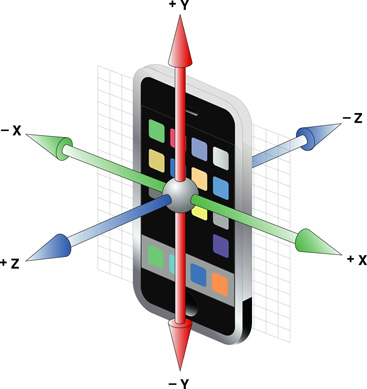
\includegraphics[width=8cm]{../img/accelerometer-axis.jpg} }}%
		\caption{The X, Y and Z axis af a smart phone device}%
		\label{fig:example}% 
	\end{figure}
	
	\begin{figure}[h]
		\centering
		\subfloat{{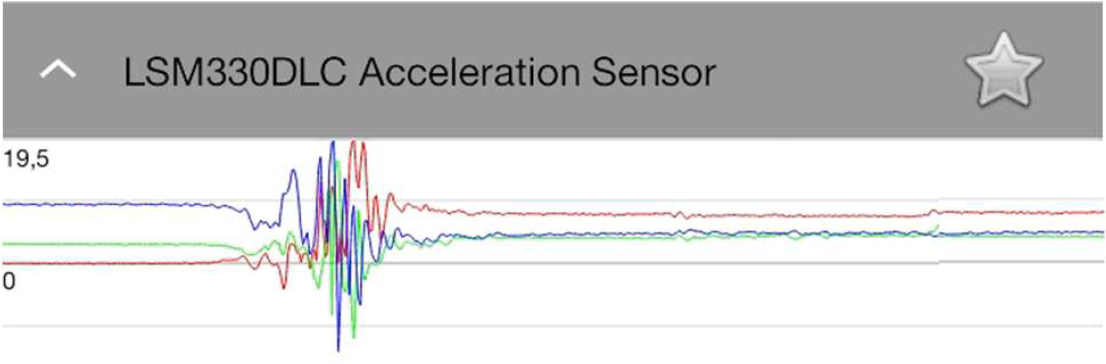
\includegraphics[width=8cm]{../img/Falling.png} }}%
		\caption{The typical pattern of falling}%
		\label{fig:example}%
	\end{figure}
	
	\noindent This measurements shows that falling, as was previously theorized, is indicated by a significant drop in acceleration towards the earth's gravitational pull, signalling that the device is moving towards a free fall state.This drop is then followed by an acceleration spike as the device hits the ground. If a person were to get seriously injured due to a fall s/he would usually remain still on the ground for a period of time. Acceleration would thus gradually go back to the normal \textit{1g} indicated by the flat line after the peak. 
	
	
	\begin{figure}[h]
		\centering
		\subfloat{{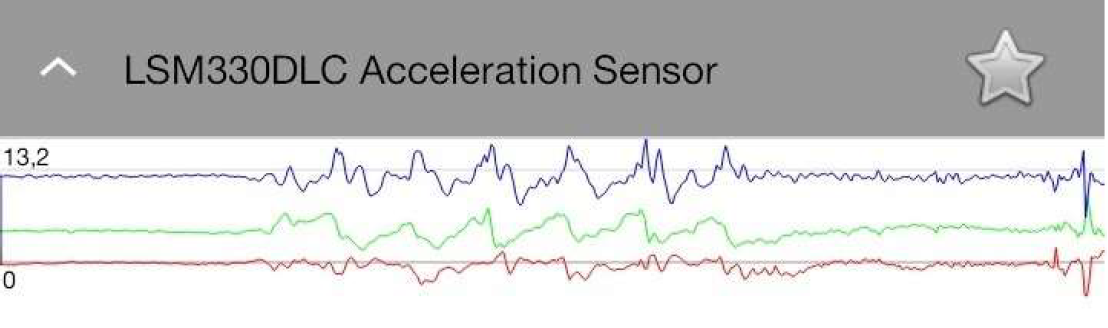
\includegraphics[width=8cm]{../img/Walking.png} }}%
		\caption{The typical pattern of walking}%
		\label{fig:example}%
	\end{figure}
	
	\noindent Walking shows a completely different pattern. As can be seen, the changes in acceleration are not rapid like the previous example. They are also repetitive, meaning that there is no longer period of non-movements after any of the peaks. The peaks them selves are also significant less than in the case of falling shown above. This implies that walking is easily distinguished from falling.
	
	
	
	\begin{figure}[h]
		\centering
		\subfloat{{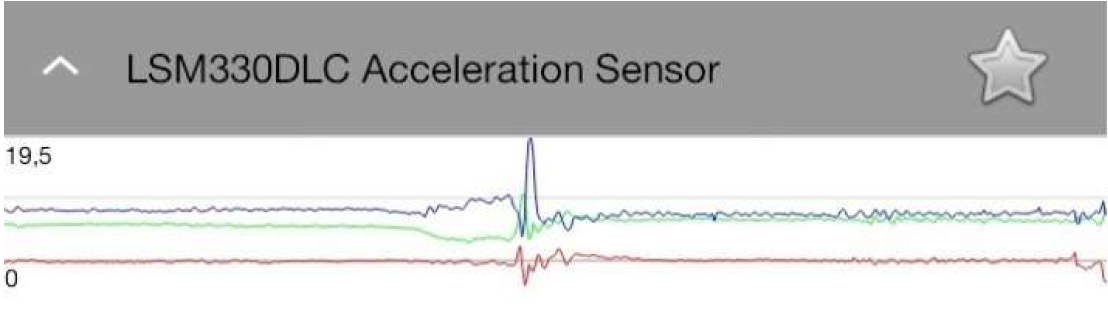
\includegraphics[width=8cm]{../img/Sitting_down.png} }}%
		\caption{The typical pattern of sitting down}%
		\label{fig:example}%
	\end{figure}
	
	\noindent Sitting down on a surface shows a similar pattern to falling with regards to a sudden drop in acceleration followed by  a rapid spike and a longer period of non-movement. The magnitude of these values are however far less than in the case of a fall and should thus be easy to single out. When a person sits down, s/he usually makes a soft movement towards the surface which is matched by the lesser accelerational  magnitude in all three directions \textit{X, Y} and \textit{Z}.
	
	
	\begin{figure}[h]
		\centering
		\subfloat{{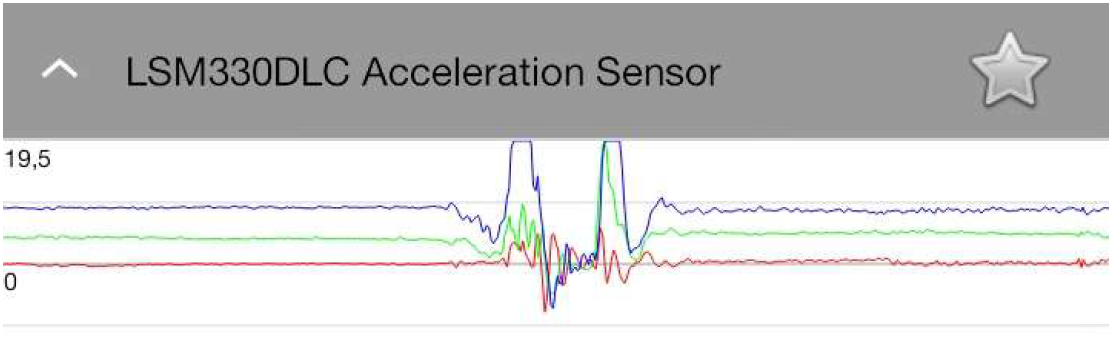
\includegraphics[width=8cm]{../img/Jumping.png} }}%
		\caption{The typical pattern of jumping}%
		\label{fig:example}%
	\end{figure}
	
	\noindent Jumping is according to Yildirim et. al. the hardest pattern to distinguish from a fall. The pattern has a sudden drop in acceleration, followed by a large spike as the jumper crouches and accelerates upwards. After this comes yet another sudden drop in acceleration as the jumper reaches the maximum altitude and starts falling back to earth again. From this part the pattern is almost identical to that of falling. When the jumper falls back to earth, the acceleration drops and then causes another huge spike as s/he hits the ground. When thinking about it, jumping and falling are in fact similar motional types, with the difference that jumping is prefixed by a drop and a spike before becoming an actual fall. The main challenge here is thus to be able to differentiate this from an unintentional falling accident.
	
	
	\paragraph{title} Abbatea et. al. takes this approach a little further by constructing 
	
	\section{Methodologies and Methods}
	
	To give an answer to the first question, what algorithm should be used, we will perform a literature study. This literature study will show which algorithm earlier work proposes.
	
	Another part of the work will be to perform a case study where the proposed algorithm will be implemented in the form of a mobile application for Android and iOS in an attempt to refine and improve the earlier work.
	
	After the mobile application is created we will perform experiments and tests to evaluate the implemented application.
	
	\subsection{Literature study}
	
	\subsection{Developing the mobile application}
	
	To develop the mobile application we will use an iterative development method. By using an iterative method we will make sure that the most important features are developed first, since we will develop the most important features in the first iteration and only after that continue with the less important features. This will help us  minimize the risks in the project. If the project would suffer from lack of time, we would at least have developed the most important features already. The project method that we will be using will be similar to Scrum, although since we are only two developers, the team involved in development will be much smaller than the typical agile team.
	
	We will divide the work in such a way that one of us will develop the Android implementation, and one of us will develop the iOS implementation. By dividing the work in this fashion we can implement similar features in both applications without the risk of writing conflicting code. Another reason for dividing the work is that it will help us to have equal focus on both the Android and iOS implementation.
	
	\subsection{Evaluating the implemented mobile application}
	
	\section{The work}
	\newpage
	
	\section{Result}
	\newpage
	
	\section{Conclusions}
	\newpage
		
	\bibliography{bib_common}
	\bibliographystyle{ieeetr}

\end{document}